\documentclass[11pt]{article}

\usepackage[margin=0.88in]{geometry}
\usepackage{amsmath,amssymb}
\usepackage{array}
\usepackage[american]{babel}
\usepackage{booktabs}
\usepackage{caption}
\usepackage{float}
\usepackage[dvipsnames]{xcolor}
\usepackage{graphicx}
\usepackage{hyperref}
\usepackage{longtable}
\usepackage{microtype}
\usepackage{ragged2e}
\usepackage{tabularx}
\usepackage{tikz}
\usepackage{url}
\usetikzlibrary{arrows.meta,positioning,fit,shapes.geometric}

\hypersetup{
colorlinks=true,
linkcolor=MidnightBlue,
citecolor=MidnightBlue,
urlcolor=MidnightBlue,
pdftitle={A Negative Result for Training-Free Whole-Prefix Visual Caching in VLA Inference},
pdfauthor={Ved Dwivedi, Cheng Yang, and Bo Yuan}
}
\setlength{\parindent}{0.22in}
\setlength{\parskip}{0.28em}
\setlength{\tabcolsep}{5pt}
\sloppy

\newcommand{\FR}{\textsc{FR}}
\newcommand{\SAVR}{\textsc{SAVR}}
\newcommand{\pp}{\,pp}
\newcommand{\code}[1]{\texttt{#1}}
\newcommand{\doi}[1]{\href{https://doi.org/#1}{doi:#1}}
\newcommand{\alt}[1]{}

\begin{document}
\justifying

\begin{center}
{\Large\bfseries A Negative Result for Training-Free Whole-Prefix\\[0.15em]
Visual Caching in VLA Inference}\\[1em]

Ved Dwivedi$^{1}$, Cheng Yang$^{2}$, and Bo Yuan$^{2}$\\[0.45em]
$^{1}$John P. Stevens High School, Edison, New Jersey\\
$^{2}$Department of Electrical and Computer Engineering, Rutgers University--New Brunswick, Piscataway, New Jersey\\[0.4em]
\textit{Preprint -- author-review version, 13 August 2026}
\end{center}

\vspace{0.6em}

\begin{abstract}
Vision-language-action (VLA) policies repeatedly encode similar observations during closed-loop manipulation, suggesting that visual features could be cached between policy queries. We study this idea through State-Aware Visual Refresh (SAVR), a training-free controller that reuses the complete projected visual prefix from a third-person and wrist camera while retaining current proprioception and the unchanged action head. The primary evaluation preserves 1,160 terminal episodes across a dense Full Refresh reference and three staged SAVR designs on one pinned OpenVLA-OFT/LIBERO-Spatial system; a separate 50-episode Full Refresh pilot measures component timing. Full Refresh succeeded on 100/100 calibration episodes. Nine initial SAVR settings achieved 0--52/100 success at 34.69--83.68\% skipped visual refreshes; the least-degrading setting still lost 48 percentage points. Offline replay underestimated online reuse for every setting. For the least-degrading setting, 374 of 783 reuse queries concealed a per-camera threshold exceedance behind the two-camera mean, including 372 wrist-camera exceedances, and the first comparable reuse changed the action hash in all 87 analyzable episodes. Reliability-constrained redesigns recovered success only by suppressing reuse: one configuration achieved 30/30 with zero reuse, while configurations at 6.72\% and 10.57\% skip achieved 29/30 and 27/30. A final post-hoc redesign achieved 69/70 at only 0.95\% skip. No tested operating point satisfied its predeclared success-efficiency gate. These bounded negative results describe a closed-loop reliability-efficiency trade-off for whole-prefix caching and motivate sensor-granular or task-aware reuse rather than treating a multi-camera visual prefix as indivisible.
\end{abstract}

\section*{Keywords}
vision-language-action models; robot manipulation; negative results; visual caching; adaptive computation; closed-loop control; inference efficiency

\section{Introduction}

Vision-language-action (VLA) models map language, images, and robot state directly to actions. RT-1 established scalable language-conditioned robotic control, and RT-2 directly incorporated web-scale vision-language knowledge into action generation~\cite{rt1,rt2}. OpenVLA released a 7B-parameter open model built from a Llama~2 language backbone and fused DINOv2/SigLIP visual features, and OpenVLA-OFT combined continuous actions, parallel decoding, and eight-action chunks to improve success and action-generation throughput~\cite{openvla,openvlaoft}. These works establish the model lineage and exact policy stack needed for this study.

Temporal redundancy offers an intuitive optimization opportunity. Adjacent robot observations often appear similar, and VLA-Cache has shown that selectively reusing minimally changed visual-token computation can accelerate VLA inference~\cite{vlacache}. Other directly relevant methods span task-aware visual-token selection, depth-guided compression, learned cache selection, model-confidence gating, and caching within iterative action generation~\cite{efficientvla,depthcache,learnedcache,gatedcache,actioncache}. The difficult question for this paper is whether a low-cost controller can identify when complete visual-prefix reuse preserves task success after its own actions begin changing the future trajectory.

We investigate the most direct version of this question: cache the complete projected prefix from both cameras and decide at each policy query whether to recompute it. State-Aware Visual Refresh (SAVR) combines image, robot-state, recent-action, and cache-age signals without changing policy weights. Our original hypothesis was that embodied signals would make whole-prefix reuse more reliable than visual similarity alone. The experiments did not support a useful operating point.

This paper reports the negative evidence rather than relaxing the gates or hiding failed variants. Across the tested OpenVLA-OFT/LIBERO-Spatial setting, permissive controllers changed actions and sharply reduced success, while conservative redesigns restored success by becoming nearly identical to dense inference. The study contributes:

\begin{enumerate}
    \item a controlled, stage-gated primary evaluation of whole-prefix visual reuse spanning 1,160 preserved terminal episodes, plus a separate 50-episode Full Refresh timing pilot;
    \item evidence that offline replay of dense trajectories underestimated the online reuse rate after cached actions changed the closed-loop trajectory;
    \item a camera-specific diagnosis showing that averaging the scene and wrist views concealed 374 threshold exceedances in 783 reuse queries;
    \item action-prefix evidence showing that the first comparable reuse changed the predicted action in 87/87 analyzable episodes; and
    \item a documented reliability-efficiency trade-off: increasingly conservative controllers recovered success but reduced reuse to zero or less than one percent.
\end{enumerate}

Our conclusion is deliberately bounded. We do not claim that visual caching is universally unreliable, that every reuse caused a failure, or that sensor-granular caching cannot work. We show that no tested \emph{whole-prefix} controller met its predeclared gate on one pinned model, suite, and seed, and we identify concrete mechanisms that future caching systems should avoid.

\section{Related Work}

\subsection{Vision-language-action policies}

RT-1 demonstrated transformer-based robotic control at scale, while RT-2 connected web-scale vision-language knowledge to robot actions~\cite{rt1,rt2}. OpenVLA made a 7B-parameter VLA and its training stack openly available~\cite{openvla}. OpenVLA-OFT adapted that model to continuous, chunked action prediction and reported strong LIBERO results~\cite{openvlaoft}. We use the released OpenVLA-OFT stack and a pinned four-suite checkpoint as the fixed policy under study. These four references define the architectural lineage and evaluated policy rather than serving as a general survey of VLA models.

\subsection{Efficient VLA inference and visual caching}

VLA efficiency can be improved at several levels. OpenVLA-OFT changes the action representation and decoder path, while EfficientVLA combines language-layer pruning, task-aware visual-token selection, and action-head feature caching~\cite{openvlaoft,efficientvla}. These sources distinguish model-path acceleration from the whole-prefix visual caching tested here.

Our study targets a narrower cost: recomputing visual features at every policy query. VLA-Cache is the closest published point of comparison; it compares adjacent visual inputs and reuses computation for selected minimally changed tokens~\cite{vlacache}. DepthCache adds depth structure and motion-adaptive auxiliary-view compression, while a learned adaptive approach jointly selects cached tokens and predicts a reuse ratio~\cite{depthcache,learnedcache}. A recent preprint augments VLA-Cache with action-token confidence, and ActionCache instead reuses intermediate states in flow-based action generation~\cite{gatedcache,actioncache}. SAVR differs in granularity: it reuses the entire projected prefix of two cameras and employs hand-designed image, state, action, and horizon gates. This coarse boundary makes the negative result informative without contradicting successful sensor-, token-, or action-level reuse.

\subsection{Closed-loop distribution shift}

An offline replay assumes the observations and actions recorded under a reference policy remain representative after the controller changes. Sequential decision problems violate this assumption because a changed action alters the later state distribution induced by the policy; this is a standard source of compounding error in imitation learning~\cite{dagger}. Our experiments directly measure the resulting gap between replay-calibrated and online reuse. This is not a general causal or off-policy-evaluation analysis, but it demonstrates why a cache controller should not treat dense-policy trajectories as a guaranteed online reliability oracle.

\section{Whole-Prefix Visual Reuse}

\subsection{Policy and cache boundary}

At policy query $t$, the pinned OpenVLA-OFT model receives a fixed language instruction $x$, a third-person image $o_t^{\mathrm{scene}}$, a wrist image $o_t^{\mathrm{wrist}}$, and the current eight-dimensional robot state $s_t$. The visual towers and projector produce an ordered projected prefix
\begin{equation}
z_t = \left[z_t^{\mathrm{scene}};z_t^{\mathrm{wrist}}\right].
\label{eq:prefix}
\end{equation}
The unchanged downstream model and continuous action head predict an $8\times 7$ action chunk,
\begin{equation}
\hat{A}_t = \pi_\theta(x,z_t,s_t).
\label{eq:policy}
\end{equation}

Full Refresh (\FR) recomputes both camera blocks at every query. Whole-prefix reuse instead supplies the last successfully refreshed prefix $z_{\tau_t}$ while still supplying current proprioception:
\begin{equation}
\tilde z_t =
\begin{cases}
z_t, & r_t=1,\\
z_{\tau_t}, & r_t=0,
\end{cases}
\qquad
\hat{A}_t=\pi_\theta(x,\tilde z_t,s_t),
\label{eq:reuse}
\end{equation}
where $r_t=1$ denotes refresh and $r_t=0$ denotes reuse. Figure~\ref{fig:boundary} shows the tested boundary. Reuse skips both visual towers and the projector; the language-model and action-head path remains unchanged.

\alt{Block diagram of the tested cache boundary. Scene and wrist images enter a refresh controller. Refresh recomputes two visual towers and the projector; reuse selects the cached complete two-camera prefix. Current robot state bypasses the cache and enters the unchanged downstream VLA and action head, which emits an eight-by-seven action chunk.}
\begin{figure}[t]
\centering
\resizebox{\linewidth}{!}{%
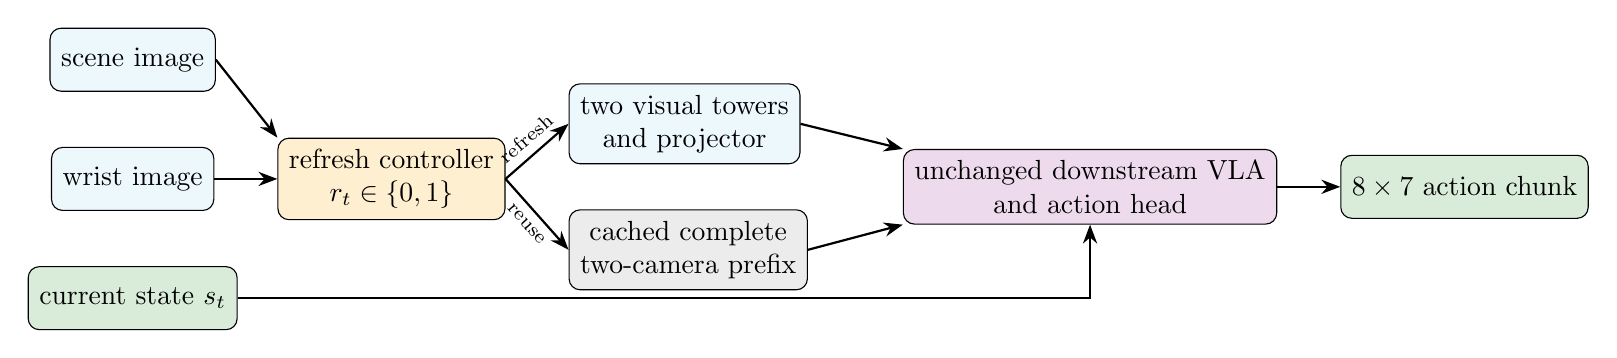
\begin{tikzpicture}[
node distance=7mm and 8mm,
box/.style={draw,rounded corners,align=center,minimum height=8mm,inner sep=4pt},
arr/.style={-{Stealth[length=2.4mm]},thick}
]
\node[box,fill=SkyBlue!15] (scene) {scene image};
\node[box,fill=SkyBlue!15,below=of scene] (wrist) {wrist image};
\node[box,fill=Green!15,below=of wrist] (state) {current state $s_t$};
\node[box,fill=Orange!18,right=of wrist] (gate) {refresh controller\\$r_t\in\{0,1\}$};
\node[box,fill=SkyBlue!15,right=of gate,yshift=7mm] (vision) {two visual towers\\and projector};
\node[box,fill=Gray!15,right=of gate,yshift=-9mm] (cache) {cached complete\\two-camera prefix};
\node[box,fill=Purple!14,right=13mm of vision,yshift=-8mm] (policy) {unchanged downstream VLA\\and action head};
\node[box,fill=Green!15,right=of policy] (action) {$8\times 7$ action chunk};
\draw[arr] (scene.east) -- (gate.north west);
\draw[arr] (wrist.east) -- (gate.west);
\draw[arr] (gate.east) -- node[above,sloped,font=\scriptsize]{refresh} (vision.west);
\draw[arr] (gate.east) -- node[below,sloped,font=\scriptsize]{reuse} (cache.west);
\draw[arr] (vision.east) -- (policy.north west);
\draw[arr] (cache.east) -- (policy.south west);
\draw[arr] (state.east) -| (policy.south);
\draw[arr] (policy.east) -- (action.west);
\end{tikzpicture}
}%
\caption{Tested whole-prefix cache boundary. A reuse skips both camera encoders and the visual projector but retains current proprioception and the complete downstream policy.}
\label{fig:boundary}
\end{figure}

\subsection{SAVR 1.0 controller}

Images were deterministically downsampled to $32\times32$ and normalized. SAVR 1.0 computed a mean absolute change for each camera relative to the last refreshed observation and then averaged the two camera scores:
\begin{equation}
d_t^{\mathrm{img}}=\frac{1}{2}\sum_{c\in\{\mathrm{scene},\mathrm{wrist}\}}
\frac{1}{N}\left\|D(o_t^c)-D(o_{\tau_t}^c)\right\|_1.
\label{eq:image}
\end{equation}
Robot-state and action-chunk dimensions were normalized using calibration $q_{0.01}$ and $q_{0.99}$ bounds. The controller computed normalized root-mean-square changes $d_t^{\mathrm{state}}$ and $d_t^{\mathrm{act}}$. It refreshed when the cache was empty, a signal was invalid, action history was incomplete, a score exceeded its threshold, or cache age reached horizon $H$:
\begin{equation}
r_t=\mathbb{I}\left[
d_t^{\mathrm{img}}>\gamma_{\mathrm{img}}\ \vee\
d_t^{\mathrm{state}}>\gamma_{\mathrm{state}}\ \vee\
d_t^{\mathrm{act}}>\gamma_{\mathrm{act}}\ \vee\
h_t\ge H\right].
\label{eq:savr1}
\end{equation}
For each target skip rate in $\{25,50,75\}\%$ and horizon in $\{2,4,8\}$, a fixed $0.001$ quantile grid over Full Refresh traces selected thresholds whose replayed skip rate was closest to target, with conservative tie breaking. All thresholds were frozen before online execution.

\subsection{Reliability-constrained redesigns}

Forensic analysis motivated SAVR 2.0. It replaced the two-camera average with independent per-camera local-change gates. Each $32\times32$ image was partitioned into an $8\times8$ grid, and the mean of the four largest patch changes formed each camera score. State was split into translation, orientation, and gripper groups; action was split into translation, rotation, and gripper groups. The controller added gripper-transition vetoes, five-query warm-up, two stable fresh queries before reuse, at most one consecutive reuse, and a hard episode-prefix reuse budget $b\in\{0.05,0.10,0.15\}$. A prospective reuse was rejected when it would make
\begin{equation}
\frac{R_t+1}{t+1}>b,
\label{eq:prefixcap}
\end{equation}
where $R_t$ is the number of completed reuses before query $t$.

SAVR 3.0 was a transparently post-hoc localized redesign. Starting from the $b=0.15$ SAVR 2.0 controller, it added a translation-direction-reversal veto and changed only the wrist-image threshold to $0.375$. It was evaluated once on states not used in the SAVR 2.0 screen.

\section{Experimental Design}

\subsection{Pinned system}

Table~\ref{tab:system} summarizes the fixed evaluation system. The base policy, checkpoint, prompt, preprocessing, action head, and simulator settings were not changed across refresh policies.

\begin{table}[H]
\centering
\scriptsize
\caption{Pinned evaluation system.}
\label{tab:system}
\begin{tabularx}{0.94\linewidth}{>{\bfseries\raggedright\arraybackslash}p{3.2cm}>{\raggedright\arraybackslash}X}
\toprule
Base policy & OpenVLA-OFT, continuous L1 action head, eight-action chunks \\
Checkpoint & \nolinkurl{openvla-7b-oft-libero-four-suite}\par Revision: \nolinkurl{638918f3d1c2e43a39a8a20772bdb8b91835e4b7} \\
OpenVLA-OFT revision & \nolinkurl{e4287e94541f459edc4feabc4e181f537cd569a8} \\
LIBERO revision & \nolinkurl{8f1084e3132a39270c3a13ebe37270a43ece2a01} \\
Benchmark & LIBERO-Spatial tasks 0--9~\cite{libero} \\
Observations & Third-person image, wrist image, current 8-D proprioception \\
Hardware & One NVIDIA TITAN RTX (24 GiB) per run \\
Primary metric & Official terminal task success \\
Efficiency proxy & Fraction of policy queries that skipped both visual towers and projector \\
\bottomrule
\end{tabularx}
\end{table}

\subsection{Populations and stage gates}

The study followed immutable stage gates rather than repeatedly tuning on the same result.

\begin{itemize}
    \item \textbf{SAVR 1.0 calibration:} 100 paired episodes per setting, covering tasks 0--9, initial states 0--9, and seed 0. Full Refresh used the same 100 task/state pairs. A setting was eligible only if all records reconciled, no technical failure occurred, no task collapsed to zero success when FR succeeded, and its paired success difference from FR was at least $-2\pp$.
    \item \textbf{SAVR 2.0 Stage 1:} three predeclared candidates, each on tasks 0--9 and states 0--2 (30 episodes). Advancement required exactly 30/30 success, at least 2\% online skip, zero technical failures, and complete cache/counter invariants.
    \item \textbf{SAVR 3.0 validation:} one frozen post-hoc controller on tasks 0--9 and states 3--9 (70 episodes). The gate required 70/70 overall, 7/7 per task, at least 5\% skip, and zero technical or accounting failures.
\end{itemize}

The final holdout (states 10--49 and seeds 7, 17, 27) was never executed or inspected because no configuration passed its preceding gate. Matched-budget Periodic Refresh and Visual-Only Refresh baselines were also not run: the frozen protocol permitted them only after an eligible SAVR 1.0 configuration existed. Consequently, this paper reports a bounded method-rejection study, not final non-inferiority or superiority.

Task-success uncertainty is summarized with two-sided 95\% exact Clopper--Pearson intervals~\cite{clopperpearson}. These intervals quantify binomial sampling uncertainty within each staged population; they do not make the distinct stage populations directly comparable.

\subsection{Correctness and integrity safeguards}

Wrapped Full Refresh produced bitwise-identical actions to the unmodified OpenVLA-OFT path. Real reuse invoked zero vision-backbone and projector calls, executed the language-model and action-head path once, and used current proprioception. Every reported rollout terminated without infrastructure failure. Scientific failures were retained rather than rerun or relabeled. Run manifests recorded configuration and source revisions, and protected checkpoint files were restored to their original hashes. Large raw records remain indexed by authenticated summaries.

\subsection{Measured optimization opportunity}

Before testing reuse, a 50-episode Full Refresh pilot measured 662 steady-state queries after three predeclared warm-ups. Table~\ref{tab:timing} shows that the visual backbone and projector accounted for 15.874\% of query CUDA time. Even perfect visual elimination therefore had a measured ceiling of approximately 15.87\% query-latency reduction before cache/controller overhead.

\begin{table}[H]
\centering
\small
\caption{Steady-state Full Refresh component timing on 662 policy queries.}
\label{tab:timing}
\begin{tabular}{lrrr}
\toprule
Component & Mean (ms) & Median (ms) & P95 (ms) \\
\midrule
Policy-query CUDA & 1267.44 & 1266.44 & 1287.80 \\
Vision backbone & 191.12 & 193.95 & 199.84 \\
Visual projector & 10.08 & 9.48 & 11.97 \\
Backbone + projector & 201.19 & 203.20 & 211.62 \\
Residual downstream & 1061.21 & 1058.79 & 1072.55 \\
\bottomrule
\end{tabular}
\end{table}

\section{Results}

\subsection{SAVR 1.0 failed throughout the tested operating region}

Full Refresh succeeded on all 100 paired calibration episodes and produced 1,309 signal traces. Table~\ref{tab:savr1} reports the complete nine-setting grid. Every SAVR 1.0 setting missed the frozen $-2\pp$ gate by a wide margin. The least-degrading setting, \code{savr-s25-h2}, achieved 52/100 success at 34.69\% online skip, a paired difference of $-48\pp$. Increasing target reuse or horizon did not reveal a success-preserving region; two settings achieved zero successes.

\begin{table}[H]
\centering
\scriptsize
\caption{Complete SAVR 1.0 online grid. Every row uses the same 100 paired task/state episodes. Brackets give two-sided 95\% exact binomial confidence intervals for success~\cite{clopperpearson}.}
\label{tab:savr1}
\begin{tabular}{lrrrrrr}
\toprule
Configuration & Target skip & $H$ & Success & 95\% CI (\%) & Online skip & Difference \\
\midrule
Full Refresh & -- & -- & 100/100 & [96.38, 100.00] & 0.00\% & $0\pp$ \\
\code{s25-h2} & 25\% & 2 & 52/100 & [41.78, 62.10] & 34.69\% & $-48\pp$ \\
\code{s25-h4} & 25\% & 4 & 21/100 & [13.49, 30.29] & 43.29\% & $-79\pp$ \\
\code{s25-h8} & 25\% & 8 & 23/100 & [15.17, 32.49] & 47.28\% & $-77\pp$ \\
\code{s50-h2} & 50\% & 2 & 12/100 & [6.36, 20.02] & 56.62\% & $-88\pp$ \\
\code{s50-h4} & 50\% & 4 & 4/100 & [1.10, 9.93] & 63.26\% & $-96\pp$ \\
\code{s50-h8} & 50\% & 8 & 0/100 & [0.00, 3.62] & 65.21\% & $-100\pp$ \\
\code{s75-h2} & 75\% & 2 & 3/100 & [0.62, 8.52] & 64.14\% & $-97\pp$ \\
\code{s75-h4} & 75\% & 4 & 1/100 & [0.03, 5.45] & 75.00\% & $-99\pp$ \\
\code{s75-h8} & 75\% & 8 & 0/100 & [0.00, 3.62] & 83.68\% & $-100\pp$ \\
\bottomrule
\end{tabular}
\end{table}

Figure~\ref{fig:frontier} places every staged operating point on a descriptive success-skip plane. Populations differ across stages, so the plot is not a randomized head-to-head comparison. Its purpose is to show the observed trade-off: high reuse accompanied low success, while high success required almost dense refresh.

\alt{Two-panel scatter plot of terminal task success versus online visual skip rate. The full panel shows Full Refresh at zero skip and 100 percent success, SAVR1 points from 34.69 to 83.68 percent skip with zero to 52 percent success, and a boxed high-success region. The expanded panel shows SAVR2 and SAVR3 points; success approaches Full Refresh only as skip approaches zero.}
\begin{figure}[t]
\centering
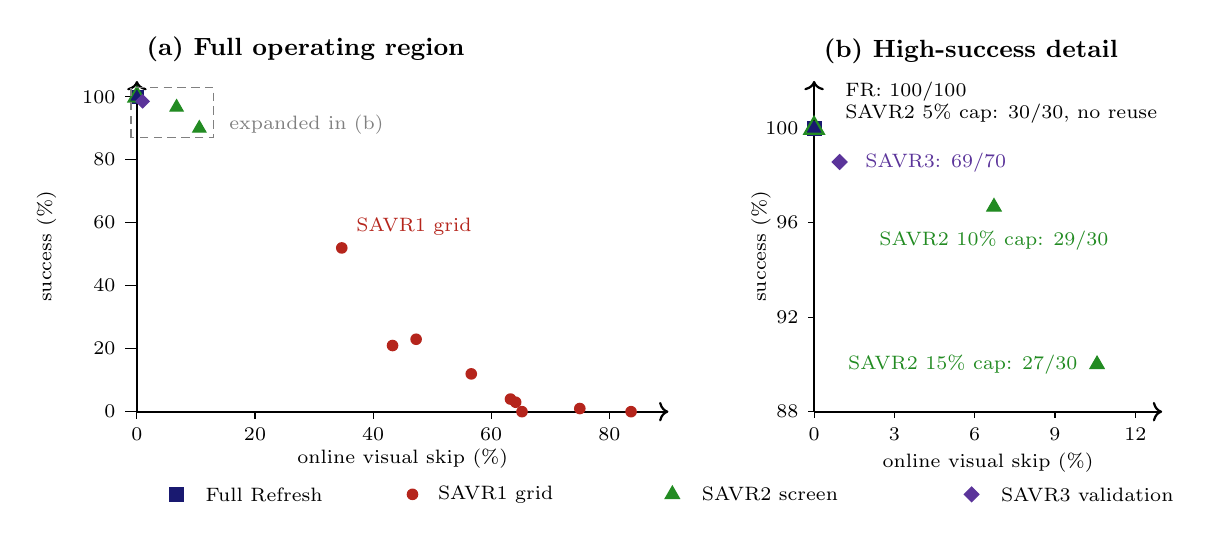
\begin{tikzpicture}[font=\scriptsize]
% Panel (a): full operating region.
\begin{scope}[x=0.075cm,y=0.040cm]
\draw[->,thick] (0,0) -- (90,0);
\draw[->,thick] (0,0) -- (0,105);
\foreach \x in {0,20,...,80}{\draw (\x,0) -- (\x,-2.2) node[below]{\x};}
\foreach \y in {0,20,...,100}{\draw (0,\y) -- (-2,\y) node[left]{\y};}
\node[anchor=south] at (45,-21) {online visual skip (\%)};
\node[rotate=90,anchor=south] at (-12,52.5) {success (\%)};
\node[font=\small\bfseries,anchor=south west] at (0,108) {(a) Full operating region};
\foreach \x/\y in {34.69/52,43.29/21,47.28/23,56.62/12,63.26/4,65.21/0,64.14/3,75/1,83.68/0}{
  \fill[BrickRed] (\x,\y) circle (2.1pt);
}
\node[anchor=south west,text=BrickRed] at (35.5,53) {SAVR1 grid};
\node[draw=MidnightBlue,fill=MidnightBlue,rectangle,minimum size=4.5pt,inner sep=0pt] at (0,100) {};
\node[draw=ForestGreen,line width=0.7pt,regular polygon,regular polygon sides=3,minimum size=7pt,inner sep=0pt] at (0,100) {};
\node[draw=ForestGreen,fill=ForestGreen,regular polygon,regular polygon sides=3,minimum size=5.5pt,inner sep=0pt] at (6.72,96.67) {};
\node[draw=ForestGreen,fill=ForestGreen,regular polygon,regular polygon sides=3,minimum size=5.5pt,inner sep=0pt] at (10.57,90) {};
\node[draw=RoyalPurple,fill=RoyalPurple,diamond,minimum size=5pt,inner sep=0pt] at (0.9534,98.57) {};
\draw[densely dashed,gray] (-1,87) rectangle (13,103);
\node[anchor=west,text=gray] at (14,91) {expanded in (b)};
\end{scope}

% Panel (b): exact-coordinate expansion of the high-success cluster.
\begin{scope}[shift={(8.6cm,0cm)},x=0.34cm,y=0.30cm]
\draw[->,thick] (0,0) -- (13,0);
\draw[->,thick] (0,0) -- (0,14);
\foreach \x in {0,3,6,9,12}{\draw (\x,0) -- (\x,-0.28) node[below]{\x};}
\foreach \y/\lab in {0/88,4/92,8/96,12/100}{\draw (0,\y) -- (-0.22,\y) node[left]{\lab};}
\node[anchor=south] at (6.5,-3.0) {online visual skip (\%)};
\node[rotate=90,anchor=south] at (-1.25,7) {success (\%)};
\node[font=\small\bfseries,anchor=south west] at (0,14.3) {(b) High-success detail};
\node[draw=MidnightBlue,fill=MidnightBlue,rectangle,minimum size=5pt,inner sep=0pt] at (0,12) {};
\node[draw=ForestGreen,line width=0.8pt,regular polygon,regular polygon sides=3,minimum size=8pt,inner sep=0pt] at (0,12) {};
\node[draw=RoyalPurple,fill=RoyalPurple,diamond,minimum size=5.5pt,inner sep=0pt] at (0.9534,10.57) {};
\node[draw=ForestGreen,fill=ForestGreen,regular polygon,regular polygon sides=3,minimum size=6pt,inner sep=0pt] at (6.72,8.67) {};
\node[draw=ForestGreen,fill=ForestGreen,regular polygon,regular polygon sides=3,minimum size=6pt,inner sep=0pt] at (10.57,2) {};
\node[anchor=west,align=left] at (0.8,13.1) {FR: 100/100\\SAVR2 5\% cap: 30/30, no reuse};
\node[anchor=west,text=RoyalPurple] at (1.55,10.55) {SAVR3: 69/70};
\node[anchor=north,text=ForestGreen] at (6.72,8.05) {SAVR2 10\% cap: 29/30};
\node[anchor=east,text=ForestGreen] at (10.2,2) {SAVR2 15\% cap: 27/30};
\end{scope}

% Shared legend, positioned in physical units below both panels.
\begin{scope}[shift={(0.5cm,-1.05cm)}]
\node[draw=MidnightBlue,fill=MidnightBlue,rectangle,minimum size=5pt,inner sep=0pt] at (0,0) {};
\node[anchor=west] at (0.25,0) {Full Refresh};
\fill[BrickRed] (3.0,0) circle (2.1pt);
\node[anchor=west] at (3.2,0) {SAVR1 grid};
\node[draw=ForestGreen,fill=ForestGreen,regular polygon,regular polygon sides=3,minimum size=6pt,inner sep=0pt] at (6.3,0) {};
\node[anchor=west] at (6.55,0) {SAVR2 screen};
\node[draw=RoyalPurple,fill=RoyalPurple,diamond,minimum size=5.5pt,inner sep=0pt] at (10.1,0) {};
\node[anchor=west] at (10.35,0) {SAVR3 validation};
\end{scope}
\end{tikzpicture}
\caption{Observed success-efficiency trade-off. Panel (b) expands the dashed region in panel (a) without moving any point. Full Refresh and the SAVR2 5\% cap coincide at 0\% skip and 100\% success; the latter made no reuse decision. SAVR1 used 100 episodes per setting, SAVR2 used 30 per setting, and SAVR3 used 70. Exact 95\% binomial confidence intervals for every success count appear in Tables~\ref{tab:savr1} and~\ref{tab:redesign}; they are not drawn here because the stages used different populations and gates. The cross-stage plot is descriptive rather than a randomized comparison.}
\label{fig:frontier}
\end{figure}

\subsection{Offline replay underestimated online reuse}

All nine settings skipped more often online than predicted by replaying Full Refresh traces. For the 25\% target family, replay predicted 24.98\% skip, while online skip reached 34.69\%, 43.29\%, and 47.28\% for horizons 2, 4, and 8, overshoots of 9.71, 18.31, and 22.30 percentage points. Once a reused prefix changed an action, later observations and controller inputs followed a different trajectory from the dense trace. The replay remained useful for screening thresholds, but it was not an online budget or reliability oracle.

\subsection{Camera averaging concealed wrist dynamics}

For \code{savr-s25-h2}, 374 of 783 reuse queries (47.77\%) had at least one camera above the shared image threshold while the two-camera average remained below it. Of these concealed exceedances, 372 came from the wrist view and only two from the third-person view. This directly invalidates cross-camera averaging as a conservative gate in this setting. It does not prove that every wrist exceedance caused an episode failure.

\subsection{The first reuse changed the predicted action}

Eighty-seven \code{savr-s25-h2} episodes had comparable Full Refresh and SAVR action hashes through their first reuse. In all 87, the first mismatch occurred exactly at the first reuse query. Ten task-4 episodes already differed at query 0 and were excluded from this comparison; three episodes never reused. The result proves immediate policy-output divergence, but action hashes do not measure magnitude and cannot alone establish that the divergence caused terminal failure.

Reuse timing and streaks were also associated with outcome. Episodes whose first reuse occurred by query 2 succeeded 7/23 (30.4\%); first reuse at queries 3--4 succeeded 18/42 (42.9\%); first reuse at query 5 or later succeeded 24/32 (75.0\%); and the three no-reuse episodes all succeeded. Every failed \code{savr-s25-h2} episode reached two consecutive reuse queries, permitting up to two eight-action chunks from stale visual features. These are exploratory associations rather than randomized causal effects.

\subsection{Reliability constraints collapsed toward Full Refresh}

Table~\ref{tab:redesign} reports the predeclared SAVR 2.0 screen and SAVR 3.0 validation. SAVR 2.0's most conservative candidate achieved 30/30 only by making no reuse decision. Candidates with useful skip rates missed the exact success gate. SAVR 3.0 recovered 69/70 success, but skipped only nine of 944 visual refreshes (0.9534\%) and missed both its success and 5\% minimum-skip gates.

\begin{table}[H]
\centering
\small
\caption{Reliability-constrained redesign results with two-sided 95\% exact binomial confidence intervals for task success~\cite{clopperpearson}. These stages used different initial-state populations and are not pooled for inference.}
\label{tab:redesign}
\begin{tabularx}{\linewidth}{lrrrrrX}
\toprule
Method & Episodes & Success & 95\% CI (\%) & Queries & Reuses / skip & Frozen gate result \\
\midrule
SAVR2-$b05$ & 30 & 30/30 & [88.43, 100.00] & 388 & 0 / 0.00\% & Failed minimum 2\% skip \\
SAVR2-$b10$ & 30 & 29/30 & [82.78, 99.92] & 461 & 31 / 6.72\% & Failed exact success \\
SAVR2-$b15$ & 30 & 27/30 & [73.47, 97.89] & 473 & 50 / 10.57\% & Failed exact success \\
SAVR3 & 70 & 69/70 & [92.30, 99.96] & 944 & 9 / 0.9534\% & Failed exact success and 5\% skip \\
\bottomrule
\end{tabularx}
\end{table}

The SAVR3 trigger audit explains the low reuse rate. Across 944 queries, wrist-image change triggered 279 times, while full-image change triggered only eight times. The two-stable-fresh requirement triggered 899 times, the prefix-budget rule 424 times, and translation reversal 412 times. Triggers can co-occur, so these counts are not additive. The controller did not fail technically; it conservatively refreshed on nearly every query.

\section{Discussion}

\subsection{A closed-loop reliability-efficiency trade-off}

The experiments reveal a consistent trade-off in the tested region. Permissive whole-prefix reuse reduced visual calls but allowed stale representations to affect many future actions. Conservative rules prevented most success-degrading reuse but also removed the intended efficiency benefit. This is not simply a threshold-selection failure: three redesign stages changed camera aggregation, local scoring, semantic grouping, temporal constraints, gripper vetoes, direction reversals, and hard budgets, yet no stage satisfied its own frozen gate.

\subsection{Why offline calibration drifted}

Dense-policy replay asks what the controller \emph{would} have done on Full Refresh observations. Online reuse asks what the controller does after its previous cached action has already changed the robot state and observation stream. The 9.71--22.30\pp{} overshoot in the 25\% family is direct evidence that these distributions differed. Future cache controllers should calibrate with bounded online data, model uncertainty under intervention, or enforce budgets that remain valid under trajectory shift.

\subsection{Multi-camera prefixes should not be treated as indivisible}

The scene camera was often stable while the wrist camera changed near the manipulated object. Averaging the two made a localized wrist change appear globally acceptable; independently gating both views then made whole-prefix reuse nearly vanish. This tension suggests a different abstraction: cache or refresh sensor blocks independently, or reuse tokens according to task relevance, rather than forcing both cameras to share one binary decision. Our study motivates this direction but does not experimentally validate it.

\subsection{Skipped visual calls are not equivalent to end-to-end speedup}

The component pilot limits the upside of any visual-only method on this stack. Visual backbone and projector work accounted for 15.874\% of query CUDA time. SAVR3 skipped 0.9534\% of those calls, corresponding to only about 0.15\% of query CUDA time under a linear zero-overhead approximation. We do not report this approximation as a measured speedup: matched end-to-end timing was not eligible after the success gate failed, and controller/cache overhead would reduce the benefit further.

\section{Limitations}

This study has several important limitations.

\begin{enumerate}
    \item It evaluates one OpenVLA-OFT checkpoint on LIBERO-Spatial, one hardware class, and seed 0. Results may not transfer to other policies, camera geometries, tasks, or real robots.
    \item The final holdout was intentionally untouched because no method passed the development gate. The results reject tested operating points but do not provide confirmatory population-level non-inferiority inference.
    \item SAVR 1.0, SAVR 2.0, and SAVR 3.0 used different staged populations. Cross-version comparisons are descriptive, not randomized paired comparisons.
    \item Matched-budget Periodic Refresh and Visual-Only Refresh were not run because the predeclared protocol required an eligible SAVR configuration first. We therefore cannot claim superiority or inferiority relative to those baselines.
    \item SAVR3 was motivated by post-hoc failure analysis. Its one-time states 3--9 evaluation was protected from further tuning, but it is not independent confirmation of a prespecified original method.
    \item Action hashes identify divergence but not action magnitude or causal responsibility for task failure. Raw SAVR 1.0 videos and contact-phase annotations were unavailable for a definitive failure taxonomy.
    \item We tested complete-prefix caching. The findings do not rule out camera-block, token-level, learned, uncertainty-aware, or model-native caching.
\end{enumerate}

\section{Reproducibility and Evidence Integrity}

The accompanying repository contains the controller, cache adapter, frozen configurations, schemas, analysis scripts, tests, decision ledger, and claim-indexed reports. Table~\ref{tab:evidence} lists the principal evidence records. Large immutable run directories remain project-local and are indexed by their manifests and summary hashes.

\begin{table}[H]
\centering
\scriptsize
\caption{Primary evidence index. Displayed SHA-256 identifiers are abbreviated for readability; the repository reports contain the complete values.}
\label{tab:evidence}
\begin{tabular}{>{\raggedright\arraybackslash}p{1.55cm}>{\raggedright\arraybackslash}p{8.05cm}>{\raggedright\arraybackslash}p{3.75cm}}
\toprule
Evidence & Repository location & Integrity identifier \\
\midrule
SAVR1 & \nolinkurl{reports/PHASE6_CALIBRATION_REPORT.md} & FR trace input \nolinkurl{c1724072...9804} \\
Diagnosis & \nolinkurl{reports/PHASE6R_A_DIAGNOSIS_REPORT.md} & \nolinkurl{9416014d...2ccf} \\
SAVR2 & \nolinkurl{reports/PHASE6R_D_STAGE1_REPORT.md} & summary \nolinkurl{61a0c9dd...a9ebe} \\
SAVR3 & \nolinkurl{reports/PHASE6S_D_VALIDATION_REPORT.md} & summary \nolinkurl{bb54eef3...d046} \\
Summary & \nolinkurl{docs/evidence/negative_results_summary.csv} & tracked with source revision \\
\bottomrule
\end{tabular}
\end{table}

All terminal task failures were retained. No threshold, success margin, or population was relaxed after observation. Technical failures were separated from scientific outcomes. Protected checkpoint files were restored, and no final-holdout outcome was inspected. These safeguards are central to the contribution: the negative result is useful only if unsuccessful trials and stopping decisions remain visible.

\subsection{Controller thresholds}

Tables~\ref{tab:savr1thresholds} and~\ref{tab:redesignthresholds} report the frozen thresholds needed to reconstruct the controllers. Values are rounded to eight decimal places for presentation; the tracked JSON configurations retain the exact decimal values. SAVR 1.0 used one quantile to set all three signal thresholds for each target/horizon pair. SAVR 2.0 and SAVR 3.0 used independent grouped thresholds, a fixed $0.90$ threshold margin, and the temporal vetoes described in Section~3.3.

\begin{table}[H]
\centering
\scriptsize
\caption{Frozen SAVR 1.0 thresholds. The exact source is \nolinkurl{configs/calibration/phase6_savr_grid.json}.}
\label{tab:savr1thresholds}
\begin{tabular}{lrrrrr}
\toprule
Configuration & Quantile & $\gamma_{\mathrm{img}}$ & $\gamma_{\mathrm{state}}$ & $\gamma_{\mathrm{act}}$ & $H$ \\
\midrule
\nolinkurl{s25-h2} & 0.691 & 0.05963525 & 0.25245324 & 0.41265356 & 2 \\
\nolinkurl{s25-h4} & 0.669 & 0.05871630 & 0.23417496 & 0.40276727 & 4 \\
\nolinkurl{s25-h8} & 0.669 & 0.05871630 & 0.23417496 & 0.40276727 & 8 \\
\nolinkurl{s50-h2} & 0.917 & 0.07900843 & 0.70789849 & 0.66859356 & 2 \\
\nolinkurl{s50-h4} & 0.871 & 0.07187330 & 0.50977447 & 0.59803563 & 4 \\
\nolinkurl{s50-h8} & 0.853 & 0.07027833 & 0.46864895 & 0.56826634 & 8 \\
\nolinkurl{s75-h2} & 1.000 & 0.14457338 & 1.04053925 & 0.95490209 & 2 \\
\nolinkurl{s75-h4} & 1.000 & 0.14457338 & 1.04053925 & 0.95490209 & 4 \\
\nolinkurl{s75-h8} & 0.996 & 0.12332860 & 1.01206082 & 0.91660479 & 8 \\
\bottomrule
\end{tabular}
\end{table}

\begin{table}[H]
\centering
\scriptsize
\caption{Frozen SAVR 2.0 and SAVR 3.0 thresholds. Columns T/O/G denote translation, orientation or rotation, and gripper groups. The exact sources are \nolinkurl{configs/calibration/phase6r_d_stage1.json} and \nolinkurl{phase6s_d_validation.json}.}
\label{tab:redesignthresholds}
\begin{tabular}{lrrrrr}
\toprule
Method & Image scene & Image wrist & State T & State O & State G \\
\midrule
SAVR2-$b05$ & 0.03562500 & 0.06380515 & 0 & 0 & 0 \\
SAVR2-$b10$ & 0.31577383 & 0.58189766 & 1.03304863 & 0.38611673 & 1.8 \\
SAVR2-$b15$ & 0.32034927 & 0.61246325 & 1.04809066 & 0.42270481 & 1.8 \\
SAVR3 & 0.32034927 & 0.37500000 & 1.04809066 & 0.42270481 & 1.8 \\
\bottomrule
\end{tabular}

\vspace{0.45em}

\begin{tabular}{lrrrr}
\toprule
Method & Action T & Action R & Action G & Budget $b$ \\
\midrule
SAVR2-$b05$ & 0.01659583 & 0.02859457 & 0 & 0.05 \\
SAVR2-$b10$ & 0.89110528 & 0.69287883 & 1.79598620 & 0.10 \\
SAVR2-$b15$ & 0.92800921 & 0.78128348 & 1.79782114 & 0.15 \\
SAVR3 & 0.92800921 & 0.78128348 & 1.79782114 & 0.15 \\
\bottomrule
\end{tabular}
\end{table}

\section{Artifact Availability and Submission Status}

The source, controller, frozen configurations, tests, and evidence audits are maintained at \url{https://github.com/vwdr/SAVR}. The repository remains private during author review, and no archival DOI exists for this revision. Before external submission, the authors will create a public, versioned archival release with a persistent identifier and will state any access restrictions on large project-local rollout records. The source includes alternative descriptions for both figures, but this format-neutral author-review PDF is not certified as tagged or PDF/UA accessible. A tagged venue-compliant PDF, the selected venue's template and page limits, disclosure language, and artifact requirements remain required before submission.

\section{Conclusion}

Training-free whole-prefix visual caching did not provide a success-preserving and useful operating point for the tested OpenVLA-OFT/LIBERO-Spatial system. Aggressive reuse changed actions and sharply reduced success; progressively stronger safeguards recovered success only by collapsing toward Full Refresh. Offline dense-trajectory replay underestimated online reuse, and a two-camera average concealed frequent wrist-camera changes. These findings do not invalidate visual caching broadly. They show that closed-loop trajectory shift, sensor-specific dynamics, and cache granularity must be treated as first-class design constraints. Reporting this trade-off prevents a failed coarse-grained design from being mistaken for evidence that visual redundancy is automatically reliable to exploit.

\begin{thebibliography}{13}

\bibitem{rt1}
A.~Brohan et al.
\newblock RT-1: Robotics Transformer for Real-World Control at Scale.
\newblock In \emph{Proceedings of Robotics: Science and Systems XIX}, 2023.
\newblock \doi{10.15607/RSS.2023.XIX.025}.

\bibitem{rt2}
B.~Zitkovich et al.
\newblock RT-2: Vision-Language-Action Models Transfer Web Knowledge to Robotic Control.
\newblock In \emph{Proceedings of the 7th Conference on Robot Learning}, PMLR 229:2165--2183, 2023.

\bibitem{openvla}
M.~J.~Kim et al.
\newblock OpenVLA: An Open-Source Vision-Language-Action Model.
\newblock In \emph{Proceedings of the 8th Conference on Robot Learning}, PMLR 270:2679--2713, 2025.

\bibitem{openvlaoft}
M.~J.~Kim, C.~Finn, and P.~Liang.
\newblock Fine-Tuning Vision-Language-Action Models: Optimizing Speed and Success.
\newblock In \emph{Proceedings of Robotics: Science and Systems XXI}, 2025.
\newblock \doi{10.15607/RSS.2025.XXI.017}.

\bibitem{efficientvla}
Y.~Yang, Y.~Wang, Z.~Wen, Z.~Luo, C.~Zou, Z.~Zhang, C.~Wen, and L.~Zhang.
\newblock EfficientVLA: Training-Free Acceleration and Compression for Vision-Language-Action Models.
\newblock \emph{Advances in Neural Information Processing Systems}, 38, 2025.

\bibitem{vlacache}
S.~Xu, Y.~Wang, C.~Xia, D.~Zhu, T.~Huang, and C.~Xu.
\newblock VLA-Cache: Efficient Vision-Language-Action Manipulation via Adaptive Token Caching.
\newblock \emph{Advances in Neural Information Processing Systems}, 38, 2025.

\bibitem{depthcache}
Y.~Li, L.~Ma, H.~Ding, and L.~Zhu.
\newblock DepthCache: Depth-Guided Training-Free Visual Token Merging for Vision-Language-Action Model Inference.
\newblock \emph{arXiv:2603.10469v1}, 2026.

\bibitem{learnedcache}
Y.~Wei, J.~Fan, J.~Guo, R.~Zhen, R.~Shao, X.~Su, Z.~Xie, and S.~Yang.
\newblock Learning to Accelerate Vision-Language-Action Models through Adaptive Visual Token Caching.
\newblock \emph{arXiv:2602.00686v1}, 2026.

\bibitem{gatedcache}
Z.~Wu, K.~Kawaharazuka, and K.~Okada.
\newblock Neural Introspection Gating for Adaptive KV-Cache Reuse in Vision-Language-Action Models.
\newblock \emph{arXiv:2608.10824v1}, 11 August 2026.

\bibitem{actioncache}
R.~Oi, H.~Otsuka, K.~Matsushima, Y.~Ichikawa, M.~Motomura, T.~Kaneko, and D.~Fujiki.
\newblock Training-Free Acceleration for Vision-Language-Action Models with Action Caching and Refinement.
\newblock \emph{arXiv:2607.06370v1}, 2026.

\bibitem{dagger}
S.~Ross, G.~Gordon, and J.~A.~Bagnell.
\newblock A Reduction of Imitation Learning and Structured Prediction to No-Regret Online Learning.
\newblock In \emph{Proceedings of the 14th International Conference on Artificial Intelligence and Statistics}, PMLR 15:627--635, 2011.

\bibitem{libero}
B.~Liu, Y.~Zhu, C.~Gao, Y.~Feng, Q.~Liu, Y.~Zhu, and P.~Stone.
\newblock LIBERO: Benchmarking Knowledge Transfer for Lifelong Robot Learning.
\newblock \emph{Advances in Neural Information Processing Systems}, 36, 2023.
\newblock \doi{10.52202/075280-1939}.

\bibitem{clopperpearson}
C.~J.~Clopper and E.~S.~Pearson.
\newblock The Use of Confidence or Fiducial Limits Illustrated in the Case of the Binomial.
\newblock \emph{Biometrika}, 26(4):404--413, 1934.
\newblock \doi{10.1093/biomet/26.4.404}.

\end{thebibliography}

\end{document}
